\documentclass[aspectratio=169,11pt]{beamer}

% ================================================================
% "TABIIY TILNI QAYTA ISHLASH" KURSI
% MA'RUZA 8 --- Ilg'or RNN arxitekturalari: GRU va LSTM
%              (d08_gru_lstm.tex)
% Arxetiplar: [A][B][C][D][E] + 4 tsikl [F][G][H][I][J][K][L] +
%             [M][N][O][P][Q][R] + ilova [S]
% Rendered slayd soni: ~45 (2-haftaning to'rtinchi ma'ruzasi; L1-L7 chuqurligi)
% Qulflangan [I3]: forget gate f_t = sigma(1.5) = 0.818
%   --- P8 (Day 9) birinchi assert manbayi (course_map hand_example).
% ================================================================

% ================================================================
% RANGLAR  (asl fayldan o'zgarishsiz)
% ================================================================
\definecolor{cnublue}{rgb}{0.07,0.14,0.62}
\definecolor{cnubluelight}{rgb}{0.18,0.30,0.72}
\definecolor{cnubluebg}{rgb}{0.90,0.92,0.97}
\definecolor{deepblue}{rgb}{0.07,0.14,0.62}
\definecolor{deepred}{rgb}{0.60,0.00,0.00}
\definecolor{deepgreen}{rgb}{0.00,0.45,0.00}
\definecolor{halfgray}{gray}{0.55}

% ================================================================
% BEAMER MAVZU --- Boadilla + maxsus footer  (asl fayldan o'zgarishsiz)
% ================================================================
\usetheme{Boadilla}

\setbeamercolor{structure}{fg=cnublue}
\setbeamercolor{frametitle}{bg=cnublue,fg=white}
\setbeamercolor{title}{bg=cnublue,fg=white}
\setbeamercolor{block title}{bg=cnublue,fg=white}
\setbeamercolor{block body}{bg=cnubluebg,fg=black}
\setbeamercolor{alerted text}{fg=deepred}
\setbeamercolor{author in head/foot}{bg=cnubluelight,fg=white}
\setbeamercolor{section in head/foot}{bg=cnublue,fg=white}
\setbeamercolor{page number in head/foot}{bg=cnubluelight,fg=white}

\setbeamertemplate{mini frame}{}
\setbeamertemplate{mini frame in current section}{}
\setbeamertemplate{mini frame in current subsection}{}
\setbeamertemplate{headline}{}
\setbeamertemplate{navigation symbols}{}

\setbeamertemplate{footline}{%
  \leavevmode%
  \hbox{%
    \begin{beamercolorbox}[wd=0.17\paperwidth,ht=2.5ex,dp=1.25ex,leftskip=0.5em]{author in head/foot}%
      \usebeamerfont{author in head/foot}\scriptsize\insertshortauthor%
    \end{beamercolorbox}%
    \begin{beamercolorbox}[wd=0.69\paperwidth,ht=2.5ex,dp=1.25ex,center]{section in head/foot}%
      \usebeamerfont{section in head/foot}%
      \scriptsize\insertsectionnavigationhorizontal{0.69\paperwidth}{}{}%
    \end{beamercolorbox}%
    \begin{beamercolorbox}[wd=0.14\paperwidth,ht=2.5ex,dp=1.25ex,rightskip=0.5em]{page number in head/foot}%
      \hfill\scriptsize\color{white}%
      \insertframenumber{}/\inserttotalframenumber%
    \end{beamercolorbox}%
  }%
  \vskip0pt%
}

% ================================================================
% PAKETLAR  (asl fayldan o'zgarishsiz)
% ================================================================
\usepackage[utf8]{inputenc}
\usepackage[T1]{fontenc}
\usepackage{lmodern}
\usepackage{amsmath,amssymb}
\usepackage{booktabs}
\usepackage{xcolor}
\usepackage{listings}
\lstset{
    language=Python,
    basicstyle=\ttfamily\scriptsize,
    keywordstyle=\bfseries\color{deepblue},
    emphstyle=\ttfamily\color{deepred},
    stringstyle=\color{deepgreen},
    commentstyle=\itshape\color{halfgray},
    numbers=left,
    numberstyle=\scriptsize\color{halfgray},
    rulesepcolor=\color{cnublue!30},
    frame=shadowbox,
    breaklines=true,
    showstringspaces=false,
    tabsize=2
}
\usepackage{tcolorbox}
\tcbuselibrary{skins}
\tcbset{
  defbox/.style={colback=cnubluebg,colframe=cnublue,
                 fonttitle=\small\bfseries\color{white},
                 attach boxed title to top left={yshift=-2mm,xshift=4mm},
                 boxed title style={colback=cnublue,colframe=cnublue}},
  warnbox/.style={colback=orange!8,colframe=orange!70!black,
                  fonttitle=\small\bfseries},
  okbox/.style={colback=green!7,colframe=green!55!black,
                fonttitle=\small\bfseries}
}
\usepackage{tikz}
\usetikzlibrary{arrows.meta,positioning}

% ================================================================
% QO'SHIMCHALAR  (asl fayldan o'zgarishsiz)
% ================================================================
\AtBeginSection[]{%
  \begin{frame}{Prezentatsiya rejasi}
    \tableofcontents[currentsection]
  \end{frame}}

\newcommand{\bunda}[1]{{\small\textbf{bunda:}\; #1}}
\newcommand{\bajarildi}{{\color{deepgreen}\large$\checkmark$}\;}

% ================================================================
% METAMA'LUMOT
% ================================================================
\title[GRU va LSTM]{Ilg'or RNN arxitekturalari: GRU va LSTM}
\subtitle{Tabiiy tilni qayta ishlash --- 8-ma'ruza}
\author[A.A.\,Abdulali]{A.A.\,Abdulali}
\date{26-iyun 2026}
\institute{11:00--12:20 \quad$\cdot$\quad mavzu \textnumero{}8}

% ================================================================
\begin{document}
% ================================================================

% ----------------------------------------------------------------
% [A] TITUL
% ----------------------------------------------------------------
\maketitle

% ================================================================
\section[Kirish]{Kirish: uzoq xotirani darvozalar bilan saqlaymiz}
% ================================================================

% ----------------------------------------------------------------
% [B] TAKRORLASH: L7 va bugungi P7
% ----------------------------------------------------------------
\begin{frame}{Takrorlash: o'tgan darsdan ikki savol}
  \begin{columns}[T]
    \begin{column}{0.49\textwidth}
      \begin{tcolorbox}[warnbox,title=1-savol]
        \small
        L7 da RNN gradienti uzoq qadamlarda \textbf{so'ndi}. Sababi nima edi?
        (Maslahat: $\tanh$ hosilasi va ko'paytma.)
      \end{tcolorbox}
    \end{column}
    \begin{column}{0.49\textwidth}
      \begin{tcolorbox}[warnbox,title=2-savol]
        \small
        Bugun ertalab P7 da RNN klassifikatori qisqa sharhlarda ishladi. Uzoq,
        kesim oxiridagi gaplarda nega qiynaladi?
      \end{tcolorbox}
    \end{column}
  \end{columns}
  \pause
  \vspace{4pt}
  \begin{columns}[T]
    \begin{column}{0.49\textwidth}
      \begin{tcolorbox}[okbox,title=1-javob]
        \small
        $\partial h_t/\partial h_{t-1}=\mathrm{diag}(1-h^2)W_h$; har bo'g'in
        $\leq 1$ $\Rightarrow$ ko'paytma \textbf{eksponensial so'nadi}.
      \end{tcolorbox}
    \end{column}
    \begin{column}{0.49\textwidth}
      \begin{tcolorbox}[okbox,title=2-javob]
        \small
        Uzoq bog'liqlik gradienti yo'qoladi $\Rightarrow$ model uzoqdagi so'zni
        \textbf{eslab qola olmaydi}. Bugun buni \textbf{darvozalar} bilan yengamiz.
      \end{tcolorbox}
    \end{column}
  \end{columns}
\end{frame}

% ----------------------------------------------------------------
% [C] MAQSADLAR
% ----------------------------------------------------------------
\begin{frame}{Siz bugungi dars oxirida quyidagilarni bajara olasiz:}
  \begin{enumerate}\setlength\itemsep{6pt}
    \item \textbf{Tushuntira olasiz:} GRU update/reset darvozalari axborot oqimini
          qanday boshqaradi.
    \item \textbf{Tushuntira olasiz:} nega LSTM xotira katagi (cell state)
          vanishing gradientni yengadi (additiv ``magistral'').
    \item \textbf{Hisoblay olasiz:} LSTM unutish darvozasini qo'lda ---
          $f_t=\sigma(1.5)\approx 0.818$.
    \item \textbf{Taqqoslay olasiz:} GRU va LSTM ni (darvoza soni, parametr,
          qachon qaysi).
  \end{enumerate}
  \vspace{4pt}
  \begin{tcolorbox}[defbox,title=Oldindan talab]
    \footnotesize
    L7 dan: RNN rekurrensiyasi, vanishing gradient. Matematikadan: sigmoid $\sigma$,
    $\tanh$, element-bo'yicha ko'paytma ($\odot$), zanjir qoidasi.
  \end{tcolorbox}
\end{frame}

% ----------------------------------------------------------------
% [D] REJA
% ----------------------------------------------------------------
\begin{frame}{Bugungi dars rejasi:}
  \begin{center}
  \small
  \begin{tabular}{c p{5.0cm} c p{3.2cm}}
    \toprule
    \textbf{Tsikl}& \textbf{Mavzu} & \textbf{Vaqt} & \textbf{Hosil bo'luvchi natija}\\
    \midrule
    1 & GRU: update/reset darvozalari & 16 daq & $z=\sigma(1)=0.731$ \\
    2 & Vanishing gradient va cell state & 18 daq & $0.9^{10}$ vs $0.42^{10}$ \\
    3 & LSTM darvozalari (forget/input/output) & 20 daq & $f_t=\sigma(1.5)=0.818$ \\
    4 & GRU va LSTM ni taqqoslash & 16 daq & parametr soni \\
    \midrule
      & Xulosa va 8-amaliyotga ko'rsatmalar & 10 daq & Ertaga nima qurishingiz \\
    \bottomrule
  \end{tabular}
  \end{center}
  \vspace{4pt}
  \begin{tcolorbox}[warnbox,title=Bu dars RNN ni ``tuzatadi'']
    \footnotesize\sloppy
    L7 ning vanishing gradient muammosini darvozali xotira bilan yengamiz.
    Bugungi $f_t=\sigma(1.5)=0.818$ ertangi P8 da \texttt{assert} bo'ladi.
  \end{tcolorbox}
\end{frame}

% ----------------------------------------------------------------
% [E] MUAMMO BIRINCHI
% ----------------------------------------------------------------
\begin{frame}{Bugungi dars uchun muammo: o'tmishni o'zgarmagan holda olib yurish}
  \begin{columns}[T]
    \begin{column}{0.50\textwidth}
      \textbf{Oddiy RNN qayerda qiynaladi:}\\[3pt]
      \small
      \begin{tcolorbox}[warnbox,title={Har qadam holatni qayta yozadi},top=2pt,bottom=2pt]
        \footnotesize
        $h_t=\tanh(W_h h_{t-1}+W_x x_t)$ --- har qadam holatni \textbf{butunlay}
        yangilaydi va $\tanh$ siqadi. Eski ma'lumot tez ``yuviladi''.
      \end{tcolorbox}
      \vspace{3pt}
      \begin{tcolorbox}[warnbox,title={Hidden o'lchamini oshirish yordam bermaydi},top=2pt,bottom=2pt]
        \footnotesize
        Muammo o'lchamda emas --- \textbf{ko'paytmali} gradient oqimida.
      \end{tcolorbox}
    \end{column}
    \begin{column}{0.46\textwidth}
      \textbf{Bugungi yechim:}\\[4pt]
      \small
      \begin{enumerate}\setlength\itemsep{4pt}
        \item \textbf{Darvozalar} (gates): nimani saqlash, nimani yangilashni
              \emph{o'rganadi}.
        \item \textbf{Cell state} (LSTM): ma'lumotni \emph{additiv} olib yuruvchi
              ``magistral''.
        \item Gradient $\tanh$ orqali emas, darvoza orqali oqadi $\Rightarrow$
              so'nmaydi.
      \end{enumerate}
      \vspace{5pt}
      \begin{tcolorbox}[okbox,top=2pt,bottom=2pt]
        \footnotesize
        Ikki arxitektura: \textbf{GRU} (soddaroq) va \textbf{LSTM} (kuchliroq).
      \end{tcolorbox}
    \end{column}
  \end{columns}
\end{frame}

% ================================================================
\section[GRU]{GRU: axborot oqimini darvozalar boshqaradi}
% ================================================================

% ----------------------------------------------------------------
% [F1] INTUITSIYA
% ----------------------------------------------------------------
\begin{frame}{Intuitsiya: eski va yangi holat orasida ``aralashtirgich''}
  \begin{columns}[T]
    \begin{column}{0.52\textwidth}
      \small
      GRU har qadamda \textbf{qancha} yangilanishni darvoza bilan boshqaradi:
      \begin{itemize}\setlength\itemsep{1pt}
        \item \textbf{update gate} $z$: eskini saqlaymizmi yoki yangilaymizmi?
        \item \textbf{reset gate} $r$: eski holatning qanchasi yangi nomzodga kiradi?
      \end{itemize}
      \vspace{4pt}
      $z\approx 0$ $\Rightarrow$ eski holat deyarli o'zgarmaydi (xotira saqlanadi).
    \end{column}
    \begin{column}{0.44\textwidth}
      \begin{tcolorbox}[okbox,top=2pt,bottom=2pt]
        \footnotesize
        Oddiy RNN har doim to'liq yangilaydi; GRU \textbf{tanlab} yangilaydi ---
        shuning uchun uzoq xotira saqlanadi.
      \end{tcolorbox}
    \end{column}
  \end{columns}
\end{frame}

% ----------------------------------------------------------------
% [G1] RASMIY TA'RIF + BUNDA
% ----------------------------------------------------------------
\begin{frame}{GRU: rasmiy ta'rif}
  \begin{tcolorbox}[defbox,title=Ta'rif: GRU katagi]
    \vspace{-0.5em}
    \begin{align*}
      z_t &= \sigma(W_z x_t + U_z h_{t-1}) &
      r_t &= \sigma(W_r x_t + U_r h_{t-1})\\
      \tilde{h}_t &= \tanh(W_h x_t + U_h(r_t \odot h_{t-1})) &
      h_t &= (1-z_t)\odot h_{t-1} + z_t \odot \tilde{h}_t
    \end{align*}
  \end{tcolorbox}
  \vspace{2pt}
  \bunda{$z_t$ --- update gate (yangilash ulushi); $r_t$ --- reset gate;
  $\tilde{h}_t$ --- nomzod holat; $\odot$ --- element-bo'yicha ko'paytma;
  $\sigma$ --- sigmoid $(0,1)$.}
  \vspace{4pt}
  \footnotesize $h_t$ --- eski $h_{t-1}$ va yangi $\tilde{h}_t$ ning
  \textbf{darvoza bilan vaznlangan} aralashmasi.
\end{frame}

% ----------------------------------------------------------------
% [H1] KELTIRIB CHIQARISH
% ----------------------------------------------------------------
\begin{frame}{Keltirib chiqarish: GRU yangilanishi qayerdan keladi?}
  \textbf{1-qadam.} Oddiy RNN: $h_t=\tanh(\ldots)$ --- har doim \textbf{to'liq}
  qayta yoziladi.
  \pause
  \textbf{2-qadam.} G'oya: eski va yangi orasida \textbf{interpolyatsiya} qilaylik:
  $$ h_t = (1-z_t)\odot h_{t-1} + z_t \odot \tilde{h}_t $$
  \pause
  \textbf{3-qadam.} $z_t$ ni \textbf{o'rganiladigan} darvoza qilamiz
  ($\sigma\in(0,1)$). $z_t\to 0$: eski saqlanadi; $z_t\to 1$: yangiga o'tadi.
  \begin{tcolorbox}[okbox,top=2pt,bottom=2pt]
    \small \textbf{Xulosa:} model \textbf{qachon} yangilashni o'zi o'rganadi ---
    uzoq xotira uchun $z_t$ kichik bo'lib qoladi.
  \end{tcolorbox}
\end{frame}

% ----------------------------------------------------------------
% [I1] QO'LDA MISOL
% ----------------------------------------------------------------
\begin{frame}{Qo'lda misol: GRU update darvozasi}
  \begin{tcolorbox}[defbox,title={1D GRU: $W_z=1$, $U_z=0$, $x_t=1.0$}]
    \small $z_t=\sigma(W_z x_t + U_z h_{t-1})=\sigma(1{\cdot}1.0 + 0)=\sigma(1.0)$.
  \end{tcolorbox}
  \vspace{0.2em}
  \begin{columns}[T]
    \begin{column}{0.52\textwidth}
      \textbf{Hisoblaymiz:} ($h_{t-1}=0.2$, $\tilde{h}_t=0.8$)
      \begin{align*}
        z_t &= \sigma(1.0) = 0.731\\
        h_t &= (1-0.731){\cdot}0.2 + 0.731{\cdot}0.8\\
            &= 0.054 + 0.585 = \mathbf{0.639}
      \end{align*}
    \end{column}
    \begin{column}{0.44\textwidth}
      \begin{tcolorbox}[okbox,top=2pt,bottom=2pt]
        \footnotesize
        $z=0.731$ $\Rightarrow$ asosan yangi nomzodga o'tdi. $z$ kichik bo'lsa edi,
        eski holat ko'proq saqlanardi.
      \end{tcolorbox}
    \end{column}
  \end{columns}
\end{frame}

% ----------------------------------------------------------------
% [J1] SIZNING VAZIFANGIZ
% ----------------------------------------------------------------
\begin{frame}{Sizning vazifangiz: kichik update darvozasi}
  \begin{tcolorbox}[warnbox,title=Savol --- 60 soniya]
    \small
    Agar $z_t=\sigma(0)=0.5$ bo'lsa ($h_{t-1}=0.2$, $\tilde{h}_t=0.8$):\\[4pt]
    \textbf{\large $h_t = ?$}
  \end{tcolorbox}
  \pause
  \begin{tcolorbox}[okbox,title=Javob]
    \small
    $h_t = (1-0.5){\cdot}0.2 + 0.5{\cdot}0.8 = 0.1 + 0.4 = \mathbf{0.5}$\\[3pt]
    \footnotesize $z=0.5$ --- eski va yangi teng aralashdi. $z\to 0$ bo'lsa
    $h_t\to h_{t-1}$ (xotira to'liq saqlanadi).
  \end{tcolorbox}
\end{frame}

% ----------------------------------------------------------------
% [K1] KOD <-> FORMULA  [fragile]
% ----------------------------------------------------------------
\begin{frame}[fragile]{Kod $\leftrightarrow$ formula: GRU katagi}
  \begin{columns}[T]
    \begin{column}{0.56\textwidth}
\begin{lstlisting}
import numpy as np

def sigmoid(x):
    return 1 / (1 + np.exp(-x))

def gru_step(h_prev, x, Wz, Uz, Wh, Uh, Wr, Ur):
    z = sigmoid(Wz*x + Uz*h_prev)
    r = sigmoid(Wr*x + Ur*h_prev)
    h_tilde = np.tanh(Wh*x + Uh*(r*h_prev))
    return (1 - z)*h_prev + z*h_tilde

print(gru_step(0.2, 1.0, 1,0, 1,0, 1,0))
\end{lstlisting}
    \end{column}
    \begin{column}{0.40\textwidth}
      \textbf{Kod $\to$ formula:}\\[3pt]
      \footnotesize
      \begin{tabular}{p{2.0cm}p{2.0cm}}
        \toprule
        Kod & Formula \\
        \midrule
        \texttt{z} & $z_t$ (update) \\
        \texttt{r} & $r_t$ (reset) \\
        \texttt{(1-z)*h+z*ht} & $h_t$ \\
        \bottomrule
      \end{tabular}
      \vspace{4pt}
      \begin{tcolorbox}[okbox,top=2pt,bottom=2pt]
        \footnotesize
        Kaggle'da \texttt{nn.GRU} buni optimal C kodda bajaradi. P8 da
        \texttt{m08} GRU ni sinaydi.
      \end{tcolorbox}
    \end{column}
  \end{columns}
\end{frame}

% ----------------------------------------------------------------
% [L1] TUZOG'
% ----------------------------------------------------------------
\begin{frame}{GRU tuzog'i: darvoza --- sehr emas}
  \begin{columns}[T]
    \begin{column}{0.52\textwidth}
      \begin{tcolorbox}[warnbox,title=Cheklovlar]
        \small
        \begin{itemize}\setlength\itemsep{2pt}
          \item GRU vanishing gradientni \textbf{yumshatadi}, butunlay yo'qotmaydi.
          \item Juda uzoq bog'liqlikda hali ham qiynalishi mumkin.
          \item Ko'proq parametr $\Rightarrow$ kichik ma'lumotda ortiqcha moslashish.
        \end{itemize}
      \end{tcolorbox}
    \end{column}
    \begin{column}{0.44\textwidth}
      \begin{tcolorbox}[okbox,top=2pt,bottom=2pt]
        \footnotesize
        \textbf{Yechim yo'nalishi:} alohida \textbf{cell state} bilan ma'lumotni
        additiv olib yurish --- LSTM (2- va 3-tsikl).
      \end{tcolorbox}
    \end{column}
  \end{columns}
\end{frame}

% ================================================================
\section[Cell state]{Vanishing gradient va cell state}
% ================================================================

% ----------------------------------------------------------------
% [F2] INTUITSIYA
% ----------------------------------------------------------------
\begin{frame}{Intuitsiya: ma'lumot uchun ``magistral yo'l''}
  \begin{columns}[T]
    \begin{column}{0.52\textwidth}
      \small
      Oddiy RNN da har qadam ma'lumotni $\tanh$ va $W_h$ orqali ``qayta ishlaydi''
      --- gradient siqiladi.\\[6pt]
      LSTM \textbf{cell state} $c_t$ ni qo'shadi: ma'lumot unga \textbf{qo'shiladi}
      (additiv), darvozalar esa nimani o'chirish/qo'shishni boshqaradi.\\[4pt]
      $c_t$ --- to'siqsiz ``magistral''; gradient bu yo'l bo'ylab so'nmasdan oqadi.
    \end{column}
    \begin{column}{0.44\textwidth}
      \begin{tcolorbox}[okbox,top=2pt,bottom=2pt]
        \footnotesize
        Tasvir: $h_t$ --- ko'cha (har burchakda to'xtash); $c_t$ --- avtomagistral
        (to'g'ridan-to'g'ri). Uzoq masofa uchun magistral kerak.
      \end{tcolorbox}
    \end{column}
  \end{columns}
\end{frame}

% ----------------------------------------------------------------
% [G2] RASMIY TA'RIF + BUNDA
% ----------------------------------------------------------------
\begin{frame}{Cell state va gradient oqimi: rasmiy ta'rif}
  \begin{tcolorbox}[defbox,title=Ta'rif: cell state yangilanishi va uning hosilasi]
    \vspace{-0.4em}
    $$ c_t = f_t \odot c_{t-1} + i_t \odot \tilde{c}_t,
       \qquad \frac{\partial c_t}{\partial c_{t-1}} = f_t $$
  \end{tcolorbox}
  \vspace{2pt}
  \bunda{$c_t$ --- xotira katagi (cell state); $f_t$ --- forget gate $(0,1)$;
  $i_t$ --- input gate; $\tilde{c}_t$ --- nomzod xotira; hosila $f_t$ --- na $W$
  matritsasi, na $\tanh$ siqilishi bor.}
  \vspace{4pt}
  \footnotesize Uzoq masofada gradient $\approx \prod_t f_t$: agar $f_t\approx 1$
  bo'lsa, gradient \textbf{so'nmaydi} --- oddiy RNN dagi $\prod(1-h^2)W_h$ dan farqli.
\end{frame}

% ----------------------------------------------------------------
% [H2] KELTIRIB CHIQARISH
% ----------------------------------------------------------------
\begin{frame}{Keltirib chiqarish: nega cell state gradientni saqlaydi?}
  \textbf{1-qadam.} Oddiy RNN: $\dfrac{\partial h_t}{\partial h_{t-1}}=\mathrm{diag}(1-h^2)\,W_h$
  --- har bo'g'in $\leq 1$, ko'paytma so'nadi.
  \pause
  \textbf{2-qadam.} LSTM cell: $c_t=f_t\odot c_{t-1}+i_t\odot\tilde{c}_t$. Bu yerda
  $c_{t-1}$ ga \textbf{matritsa ko'paytma yo'q}, faqat $f_t$ ga ko'paytiriladi:
  $$ \frac{\partial c_t}{\partial c_{t-1}} = f_t $$
  \pause
  \textbf{3-qadam.} Uzoq masofa gradienti $\approx \prod_t f_t$. $f_t\approx 1$
  bo'lsa, ko'paytma $\approx 1$ --- gradient \textbf{saqlanadi}.
  \begin{tcolorbox}[okbox,top=2pt,bottom=2pt]
    \small \textbf{Xulosa:} additiv cell state + forget gate $\approx 1$ ---
    LSTM ning vanishing gradientga qarshi asosiy hiylasi.
  \end{tcolorbox}
\end{frame}

% ----------------------------------------------------------------
% [I2] QO'LDA MISOL
% ----------------------------------------------------------------
\begin{frame}{Qo'lda misol: 10 qadamda gradient --- RNN vs LSTM}
  \begin{tcolorbox}[defbox,title={Taqqoslash: 10 qadamli ketma-ketlik}]
    \small RNN bo'g'ini $\approx 1-h^2=0.42$ (L7); LSTM forget gate $f_t=0.9$.
  \end{tcolorbox}
  \vspace{0.2em}
  \begin{columns}[T]
    \begin{column}{0.50\textwidth}
      \textbf{Oddiy RNN:}
      $$ 0.42^{10} \approx 1.7\times 10^{-4} $$
      Gradient deyarli \alert{nol} --- uzoq bog'liqlik yo'qoladi.
    \end{column}
    \begin{column}{0.46\textwidth}
      \textbf{LSTM cell ($f=0.9$):}
      $$ 0.9^{10} \approx \mathbf{0.349} $$
      Gradient \textbf{saqlanadi} --- 10 qadam uzoqlik ham ko'rinadi.
    \end{column}
  \end{columns}
  \vspace{4pt}
  \begin{tcolorbox}[okbox,top=2pt,bottom=2pt]
    \footnotesize
    $1.7\times10^{-4}$ va $0.349$ --- ikki tartibdan ko'p farq. Mana shu farq
    LSTM ni uzoq matnlarda ishlatadi.
  \end{tcolorbox}
\end{frame}

% ----------------------------------------------------------------
% [J2] SIZNING VAZIFANGIZ
% ----------------------------------------------------------------
\begin{frame}{Sizning vazifangiz: 5 qadamli gradient}
  \begin{tcolorbox}[warnbox,title=Savol --- 60 soniya]
    \small
    LSTM forget gate $f=0.9$, ketma-ketlik \textbf{5} qadam:\\[4pt]
    \textbf{\large $\prod f = 0.9^5 = ?$ \quad (taxminan)}
  \end{tcolorbox}
  \pause
  \begin{tcolorbox}[okbox,title=Javob]
    \small
    $0.9^5 = 0.59049 \approx \mathbf{0.59}$\\[3pt]
    \footnotesize Oddiy RNN da $0.42^5\approx 0.013$ bo'lardi. LSTM qisqa masofada
    ham gradientni ancha yaxshi saqlaydi.
  \end{tcolorbox}
\end{frame}

% ----------------------------------------------------------------
% [K2] KOD <-> FORMULA  [fragile]
% ----------------------------------------------------------------
\begin{frame}[fragile]{Kod $\leftrightarrow$ formula: cell state oqimi}
  \begin{columns}[T]
    \begin{column}{0.56\textwidth}
\begin{lstlisting}
import numpy as np

# gradient oqimi: RNN vs LSTM cell (10 qadam)
rnn_factor  = 0.42      # ~ (1 - h^2)
lstm_forget = 0.9       # forget gate

rnn_grad  = rnn_factor ** 10
lstm_grad = lstm_forget ** 10

print("RNN :", rnn_grad)    # 1.7e-04
print("LSTM:", lstm_grad)   # 0.349
\end{lstlisting}
    \end{column}
    \begin{column}{0.40\textwidth}
      \textbf{Kod $\to$ formula:}\\[3pt]
      \footnotesize
      \begin{tabular}{p{1.9cm}p{2.1cm}}
        \toprule
        Kod & Formula \\
        \midrule
        \texttt{0.42**10} & $\prod(1-h^2)$ \\
        \texttt{0.9**10} & $\prod f_t$ \\
        \bottomrule
      \end{tabular}
      \vspace{4pt}
      \begin{tcolorbox}[warnbox,top=2pt,bottom=2pt]
        \footnotesize
        Bu soddalashtirilgan model: amalda $f_t$ har qadam o'zgaradi, ammo g'oya
        bir xil --- additiv yo'l so'nishni kamaytiradi.
      \end{tcolorbox}
    \end{column}
  \end{columns}
\end{frame}

% ----------------------------------------------------------------
% [L2] TUZOG'
% ----------------------------------------------------------------
\begin{frame}{Cell state tuzog'i: forget gate $0$ ga tushsa, xotira o'chadi}
  \begin{columns}[T]
    \begin{column}{0.52\textwidth}
      \begin{tcolorbox}[warnbox,title=Forget gate ikki yoqlama]
        \small
        $f_t\approx 1$: xotira saqlanadi (yaxshi). $f_t\approx 0$: cell state
        \textbf{tozalanadi} --- ba'zan kerak (yangi jumla), ba'zan ziyon.
        Modelni to'g'ri o'qitish muhim.
      \end{tcolorbox}
    \end{column}
    \begin{column}{0.44\textwidth}
      \begin{tcolorbox}[okbox,top=2pt,bottom=2pt]
        \footnotesize
        Amaliy maslahat: forget gate bias'ini musbat (masalan $+1$) boshlash ---
        boshida xotirani saqlashga moyil qiladi (o'qitishni tezlashtiradi).
      \end{tcolorbox}
    \end{column}
  \end{columns}
\end{frame}

% ================================================================
\section[LSTM]{LSTM darvozalari: forget, input, output}
% ================================================================

% ----------------------------------------------------------------
% [F3] INTUITSIYA
% ----------------------------------------------------------------
\begin{frame}{Intuitsiya: uchta darvoza --- o'chir, yoz, o'qi}
  \begin{columns}[T]
    \begin{column}{0.52\textwidth}
      \small
      LSTM cell state'ni \textbf{uch} darvoza boshqaradi:
      \begin{itemize}\setlength\itemsep{1pt}
        \item \textbf{forget} $f_t$: eski xotiradan nimani \emph{o'chirish}.
        \item \textbf{input} $i_t$: yangi ma'lumotdan nimani \emph{yozish}.
        \item \textbf{output} $o_t$: xotiradan nimani \emph{o'qib} chiqarish ($h_t$ ga).
      \end{itemize}
      \vspace{4pt}
      Har biri $\sigma\in(0,1)$ --- ``yarim ochiq eshik''.
    \end{column}
    \begin{column}{0.44\textwidth}
      \begin{tcolorbox}[okbox,top=2pt,bottom=2pt]
        \footnotesize
        Darvozalar --- \textbf{o'rganiladigan} filtrlar. Model qaysi ma'lumot
        muhimligini ma'lumotdan o'rganadi.
      \end{tcolorbox}
    \end{column}
  \end{columns}
\end{frame}

% ----------------------------------------------------------------
% [G3] RASMIY TA'RIF + BUNDA
% ----------------------------------------------------------------
\begin{frame}{LSTM: rasmiy ta'rif}
  \begin{tcolorbox}[defbox,title=Ta'rif: LSTM katagi]
    \vspace{-0.5em}
    \begin{align*}
      f_t &= \sigma(W_f[h_{t-1},x_t]+b_f) &
      i_t &= \sigma(W_i[h_{t-1},x_t]+b_i)\\
      o_t &= \sigma(W_o[h_{t-1},x_t]+b_o) &
      \tilde{c}_t &= \tanh(W_c[h_{t-1},x_t]+b_c)\\
      c_t &= f_t\odot c_{t-1}+i_t\odot\tilde{c}_t &
      h_t &= o_t\odot\tanh(c_t)
    \end{align*}
  \end{tcolorbox}
  \vspace{1pt}
  \bunda{$[h_{t-1},x_t]$ --- birlashtirilgan vektor; $f_t,i_t,o_t$ --- forget,
  input, output darvozalari; $c_t$ --- cell state; $h_t$ --- yashirin holat
  (chiqish).}
\end{frame}

% ----------------------------------------------------------------
% [H3] KELTIRIB CHIQARISH
% ----------------------------------------------------------------
\begin{frame}{Keltirib chiqarish: forget gate qanday ishlaydi?}
  \textbf{1-qadam.} Darvoza --- $(0,1)$ oralig'idagi ``ulush''. Sigmoid aynan shuni
  beradi: $\sigma(\cdot)\in(0,1)$.
  \pause
  \textbf{2-qadam.} Forget gate kirish va oldingi holatdan hisoblanadi:
  $$ f_t = \sigma(W_f[h_{t-1},x_t]+b_f) $$
  \pause
  \textbf{3-qadam.} U cell state'ga element-bo'yicha ko'paytiriladi: $f_t\odot c_{t-1}$.
  $f_t$ komponenti $1$ ga yaqin --- shu xotira saqlanadi; $0$ ga yaqin --- o'chiriladi.
  \begin{tcolorbox}[okbox,top=2pt,bottom=2pt]
    \small \textbf{Xulosa:} forget gate --- har bir xotira o'lchami uchun alohida
    ``saqlash darajasi''. Endi uni qo'lda hisoblaymiz.
  \end{tcolorbox}
\end{frame}

% ----------------------------------------------------------------
% [I3] QO'LDA HISOB --- QULFLANGAN TRACEABILITY SLAYD
%
% P8 (Day 9) birinchi assert bilan solishtiring:
%   forget gate f_t = sigma(1.5) = 0.818   [Ma'ruza L8 [I3]-slayd]
% course_map.yaml hand_example verbatim.
% ----------------------------------------------------------------
\begin{frame}{Qo'lda hisob: LSTM forget gate --- $f_t=\sigma(1.5)=0.818$}
  \begin{tcolorbox}[defbox,title={1D LSTM: $W_f=1$, $b_f=0$, $h_{t-1}=0.5$, $x_t=1.0$}]
    \small $f_t=\sigma(W_f h_{t-1} + W_f x_t + b_f)$ (bir o'lchamli, soddalashtirilgan).
  \end{tcolorbox}
  \vspace{0.2em}
  \begin{columns}[T]
    \begin{column}{0.54\textwidth}
      \textbf{Hisoblaymiz:}
      \begin{align*}
        f_t &= \sigma(1{\cdot}0.5 + 1{\cdot}1.0 + 0)\\
            &= \sigma(1.5) = \frac{1}{1+e^{-1.5}}\\
            &= \frac{1}{1+0.223} \approx \mathbf{0.818}
      \end{align*}
    \end{column}
    \begin{column}{0.42\textwidth}
      \begin{tcolorbox}[okbox,top=2pt,bottom=2pt]
        \footnotesize
        $f_t=0.818$ ($1$ ga yaqin) $\Rightarrow$ o'tmish holatining
        \textbf{ko'p qismi saqlanadi}.
      \end{tcolorbox}
      \vspace{3pt}
      \footnotesize\color{halfgray}
      Ertangi P8 birinchi assert:\\
      \texttt{abs(f\_t - 0.818) < 1e-3}\\
      \textit{\# Ma'ruza L8 [I3]-slayd}
    \end{column}
  \end{columns}
\end{frame}

% ----------------------------------------------------------------
% [J3] SIZNING VAZIFANGIZ
% ----------------------------------------------------------------
\begin{frame}{Sizning vazifangiz: cell state'ni yangilang}
  \begin{tcolorbox}[warnbox,title=Savol --- 90 soniya]
    \small
    $f_t=0.818$, $c_{t-1}=1.0$, input gate $i_t=0.5$, nomzod $\tilde{c}_t=0.6$:\\[4pt]
    \textbf{\large $c_t = f_t\,c_{t-1} + i_t\,\tilde{c}_t = ?$}
  \end{tcolorbox}
  \pause
  \begin{tcolorbox}[okbox,title=Javob]
    \small
    $c_t = 0.818{\cdot}1.0 + 0.5{\cdot}0.6 = 0.818 + 0.30 = \mathbf{1.118}$\\[3pt]
    \footnotesize Eski xotiradan $0.818$ saqlandi, yangidan $0.30$ qo'shildi ---
    additiv yangilanish (cell state ``magistral''i).
  \end{tcolorbox}
\end{frame}

% ----------------------------------------------------------------
% [K3] KOD <-> FORMULA  [fragile]
% ----------------------------------------------------------------
\begin{frame}[fragile]{Kod $\leftrightarrow$ formula: LSTM katagi}
  \begin{columns}[T]
    \begin{column}{0.58\textwidth}
\begin{lstlisting}
import numpy as np
def sigmoid(x): return 1/(1+np.exp(-x))

def lstm_step(h, c, x, Wf, Wi, Wo, Wc):
    z = np.array([h, x])
    f = sigmoid(Wf @ z)            # forget
    i = sigmoid(Wi @ z)            # input
    o = sigmoid(Wo @ z)            # output
    c_tilde = np.tanh(Wc @ z)
    c = f*c + i*c_tilde            # cell state
    h = o*np.tanh(c)
    return h, c

# Wf=[1,1] -> f = sigmoid(0.5+1.0) = 0.818
\end{lstlisting}
    \end{column}
    \begin{column}{0.38\textwidth}
      \textbf{Kod $\to$ formula:}\\[3pt]
      \footnotesize
      \begin{tabular}{p{1.6cm}p{2.0cm}}
        \toprule
        Kod & Formula \\
        \midrule
        \texttt{f} & $f_t$ (forget) \\
        \texttt{i} & $i_t$ (input) \\
        \texttt{f*c+i*ct} & $c_t$ \\
        \texttt{o*tanh(c)} & $h_t$ \\
        \bottomrule
      \end{tabular}
      \vspace{4pt}
      \begin{tcolorbox}[okbox,top=2pt,bottom=2pt]
        \footnotesize
        Kaggle'da \texttt{nn.LSTM}; P8 da \texttt{m08} uni GRU bilan taqqoslaydi.
      \end{tcolorbox}
    \end{column}
  \end{columns}
\end{frame}

% ----------------------------------------------------------------
% [L3] TUZOG'
% ----------------------------------------------------------------
\begin{frame}{LSTM tuzog'i: kuch --- narx bilan keladi}
  \begin{columns}[T]
    \begin{column}{0.52\textwidth}
      \begin{tcolorbox}[warnbox,title=Hisoblash narxi]
        \small
        \begin{itemize}\setlength\itemsep{2pt}
          \item 4 ta darvoza/nomzod $\Rightarrow$ oddiy RNN dan $\sim 4\times$ ko'p
                parametr.
          \item Kichik ma'lumotda ortiqcha moslashish xavfi.
          \item Sekinroq o'qiydi (ko'proq hisob).
        \end{itemize}
      \end{tcolorbox}
    \end{column}
    \begin{column}{0.44\textwidth}
      \begin{tcolorbox}[okbox,top=2pt,bottom=2pt]
        \footnotesize
        \textbf{Yechim:} kam ma'lumotda GRU (kamroq parametr) ko'pincha yetarli
        --- keyingi tsiklda taqqoslaymiz.
      \end{tcolorbox}
    \end{column}
  \end{columns}
\end{frame}

% ================================================================
\section[Taqqoslash]{GRU va LSTM ni taqqoslash}
% ================================================================

% ----------------------------------------------------------------
% [F4] INTUITSIYA
% ----------------------------------------------------------------
\begin{frame}{Intuitsiya: bir xil g'oya, ikki ``vazn toifasi''}
  \begin{columns}[T]
    \begin{column}{0.52\textwidth}
      \small
      Ikkalasi ham darvozalar bilan uzoq xotirani saqlaydi:
      \begin{itemize}\setlength\itemsep{1pt}
        \item \textbf{LSTM}: alohida cell state, 3 darvoza --- kuchliroq, og'irroq.
        \item \textbf{GRU}: cell state yo'q (h birlashgan), 2 darvoza --- yengilroq, tezroq.
      \end{itemize}
      \vspace{4pt}
      Ko'p vazifada natijalari yaqin --- tanlov ma'lumot va resursga bog'liq.
    \end{column}
    \begin{column}{0.44\textwidth}
      \begin{tcolorbox}[okbox,top=2pt,bottom=2pt]
        \footnotesize
        Amaliy qoida: kam ma'lumot/tez kerak $\Rightarrow$ GRU; ko'p ma'lumot/uzoq
        bog'liqlik $\Rightarrow$ LSTM dan boshlang.
      \end{tcolorbox}
    \end{column}
  \end{columns}
\end{frame}

% ----------------------------------------------------------------
% [G4] RASMIY TA'RIF + BUNDA
% ----------------------------------------------------------------
\begin{frame}{Parametr soni: rasmiy taqqoslash}
  \begin{tcolorbox}[defbox,title=Ta'rif: gated RNN parametrlari soni]
    \vspace{-0.4em}
    $$ \text{LSTM} \approx 4\,(d{\cdot}H + H{\cdot}H + H), \qquad
       \text{GRU} \approx 3\,(d{\cdot}H + H{\cdot}H + H) $$
  \end{tcolorbox}
  \vspace{2pt}
  \bunda{$d$ --- kirish o'lchami; $H$ --- yashirin o'lcham; $4$ --- LSTM ning
  4 ta o'zgartirishi (f,i,o,$\tilde{c}$); $3$ --- GRU ning 3 tasi (z,r,$\tilde{h}$);
  $+H$ --- bias.}
  \vspace{4pt}
  \footnotesize Demak GRU $\approx \tfrac{3}{4}$ LSTM parametri --- shuning uchun
  tezroq va kam ma'lumotda barqarorroq.
\end{frame}

% ----------------------------------------------------------------
% [H4] KELTIRIB CHIQARISH
% ----------------------------------------------------------------
\begin{frame}{Keltirib chiqarish: nega GRU kamroq parametr?}
  \textbf{1-qadam.} Har darvoza/nomzod bitta og'irlik to'plamiga ega:
  $d{\cdot}H$ (kirish) $+ H{\cdot}H$ (holat) $+ H$ (bias).
  \pause
  \textbf{2-qadam.} LSTM da bunday \textbf{4} ta blok bor ($f,i,o,\tilde{c}$); GRU da
  \textbf{3} ta ($z,r,\tilde{h}$).
  \pause
  \textbf{3-qadam.} Demak nisbat:
  $$ \frac{\text{GRU}}{\text{LSTM}} = \frac{3}{4} = 0.75 $$
  \begin{tcolorbox}[okbox,top=2pt,bottom=2pt]
    \small \textbf{Xulosa:} GRU LSTM parametrlarining $\sim$75\% i --- arzonroq,
    lekin cell state'siz (biroz kamroq ifoda kuchi).
  \end{tcolorbox}
\end{frame}

% ----------------------------------------------------------------
% [I4] QO'LDA MISOL
% ----------------------------------------------------------------
\begin{frame}{Qo'lda misol: parametr sonini sanaymiz}
  \begin{tcolorbox}[defbox,title={Kichik model: $d=2$, $H=2$}]
    \small Bitta blok: $d{\cdot}H + H{\cdot}H + H = 2{\cdot}2 + 2{\cdot}2 + 2 = 10$.
  \end{tcolorbox}
  \vspace{0.2em}
  \begin{columns}[T]
    \begin{column}{0.50\textwidth}
      \textbf{Hisoblaymiz:}
      \begin{align*}
        \text{LSTM} &= 4\times 10 = \mathbf{40}\\
        \text{GRU}  &= 3\times 10 = \mathbf{30}
      \end{align*}
    \end{column}
    \begin{column}{0.46\textwidth}
      \begin{tcolorbox}[okbox,top=2pt,bottom=2pt]
        \footnotesize
        GRU $30$ vs LSTM $40$ parametr --- $25\%$ kam. Katta $H$ da bu farq
        absolyut sonda kattalashadi.
      \end{tcolorbox}
    \end{column}
  \end{columns}
\end{frame}

% ----------------------------------------------------------------
% [J4] SIZNING VAZIFANGIZ
% ----------------------------------------------------------------
\begin{frame}{Sizning vazifangiz: kattaroq model uchun parametr}
  \begin{tcolorbox}[warnbox,title=Savol --- 90 soniya]
    \small
    $d=3$, $H=2$ uchun bitta blok $= 3{\cdot}2 + 2{\cdot}2 + 2 = 12$.\\[4pt]
    \textbf{\large LSTM va GRU parametrlari soni qancha?}
  \end{tcolorbox}
  \pause
  \begin{tcolorbox}[okbox,title=Javob]
    \small
    LSTM $= 4\times 12 = \mathbf{48}$; \quad GRU $= 3\times 12 = \mathbf{36}$.\\[3pt]
    \footnotesize Nisbat hamon $36/48 = 0.75$ --- darvoza bloklari soni farqi
    (3 vs 4) saqlanadi.
  \end{tcolorbox}
\end{frame}

% ----------------------------------------------------------------
% [K4] KOD <-> FORMULA  [fragile]
% ----------------------------------------------------------------
\begin{frame}[fragile]{Kod $\leftrightarrow$ formula: PyTorch \texttt{nn.LSTM} / \texttt{nn.GRU}}
  \begin{columns}[T]
    \begin{column}{0.58\textwidth}
\begin{lstlisting}
import torch.nn as nn

# bir xil interfeys, faqat qatlam nomi farq qiladi
lstm = nn.LSTM(input_size=100, hidden_size=128,
               batch_first=True)
gru  = nn.GRU(input_size=100, hidden_size=128,
              batch_first=True)

def n_params(m):
    return sum(p.numel() for p in m.parameters())

print("LSTM:", n_params(lstm))   # ~117k
print("GRU :", n_params(gru))    # ~88k  (~0.75x)
\end{lstlisting}
    \end{column}
    \begin{column}{0.38\textwidth}
      \textbf{Kod $\to$ formula:}\\[3pt]
      \footnotesize
      \begin{tabular}{p{1.7cm}p{1.9cm}}
        \toprule
        Kod & Formula \\
        \midrule
        \texttt{nn.LSTM} & 4 blok \\
        \texttt{nn.GRU} & 3 blok \\
        \texttt{n\_params} & $\approx 0.75\times$ \\
        \bottomrule
      \end{tabular}
      \vspace{4pt}
      \begin{tcolorbox}[okbox,top=2pt,bottom=2pt]
        \footnotesize
        P8 da \texttt{m08} aynan shu ikki qatlamni bir xil vazifada taqqoslaydi
        (\texttt{compare\_report}).
      \end{tcolorbox}
    \end{column}
  \end{columns}
\end{frame}

% ----------------------------------------------------------------
% [L4] TUZOG'
% ----------------------------------------------------------------
\begin{frame}{Taqqoslash tuzog'i: ``qaysi yaxshi'' --- noto'g'ri savol}
  \begin{columns}[T]
    \begin{column}{0.52\textwidth}
      \begin{tcolorbox}[warnbox,title=Kontekstga bog'liq]
        \small
        Universal g'olib yo'q. Natija ma'lumot hajmi, ketma-ketlik uzunligi va
        hisoblash byudjetiga bog'liq. Bittasini ``har doim yaxshi'' deyish xato.
      \end{tcolorbox}
    \end{column}
    \begin{column}{0.44\textwidth}
      \begin{tcolorbox}[okbox,top=2pt,bottom=2pt]
        \footnotesize
        \textbf{To'g'ri yondashuv:} ikkalasini bir xil vazifada sinab, F1 va
        tezlikni \textbf{o'lchang} --- aynan P8 da \texttt{compare\_report} qiladi.
      \end{tcolorbox}
    \end{column}
  \end{columns}
\end{frame}

% ================================================================
\section[Xulosa]{Xulosa va amaliyotga ko'prik}
% ================================================================

% ----------------------------------------------------------------
% [M] O'ZBEK TILIGA XOSLIK (majburiy arxetip)
% ----------------------------------------------------------------
\begin{frame}{O'zbek tilida: cell state uzun qo'shimcha zanjirini ushlay oladimi?}
  \begin{columns}[T]
    \begin{column}{0.50\textwidth}
      \textbf{1. Uzun qo'shimcha zanjiri:}\\[3pt]
      \small
      \texttt{o'rgan-il-gan-lar-dan} --- bir so'z, $\approx 4$ morfema. Token yoki
      morfema darajasida bu uzun bog'liqlik.
      \begin{tcolorbox}[okbox,title=LSTM afzalligi,top=2pt,bottom=2pt]
        \footnotesize
        Cell state morfema zanjiri davomida ma'noni \textbf{saqlay} oladi ---
        oddiy RNN dan ustun.
      \end{tcolorbox}
    \end{column}
    \begin{column}{0.46\textwidth}
      \textbf{2. SOV --- kesim oxirida:}\\[3pt]
      \small
      \textit{``men kitobni do'stimga berdim''} --- kesim uzoqda. LSTM cell state
      gap boshini oxirigacha eslab qola oladi.\\[4pt]
      \begin{tcolorbox}[warnbox,title=Lekin,top=2pt,bottom=2pt]
        \footnotesize
        O'zbek korpuslari kichik $\Rightarrow$ LSTM ortiqcha moslashishi mumkin;
        GRU (kamroq parametr) ko'pincha barqarorroq.
      \end{tcolorbox}
    \end{column}
  \end{columns}
\end{frame}

% ----------------------------------------------------------------
% [N] SINTEZ
% ----------------------------------------------------------------
\begin{frame}{Sintez: RNN, GRU, LSTM ni taqqoslaymiz}
  \begin{center}\small
  \begin{tabular}{p{2.4cm}p{1.8cm}p{2.4cm}p{3.0cm}}
    \toprule
    \textbf{Model} & \textbf{Darvoza} & \textbf{Parametr} & \textbf{Vanishing'ga qarshilik} \\
    \midrule
    Oddiy RNN & 0 & eng kam & zaif ($\prod(1-h^2)$) \\
    GRU & 2 (z, r) & $\sim 0.75\times$ LSTM & yaxshi \\
    \textbf{LSTM} & \textbf{3} (f, i, o) & eng ko'p & \textbf{eng yaxshi} (cell state) \\
    \bottomrule
  \end{tabular}
  \end{center}
  \vspace{4pt}
  \begin{tcolorbox}[okbox,title=Asosiy g'oya,top=2pt,bottom=2pt]
    \footnotesize
    Darvozalar axborot oqimini \textbf{o'rganiladigan} tarzda boshqaradi; LSTM
    cell state additiv ``magistral'' bilan gradientni saqlaydi. GRU --- shu g'oyaning
    yengil varianti. Tanlov vazifaga bog'liq.
  \end{tcolorbox}
\end{frame}

% ----------------------------------------------------------------
% [O] SEMINAL MANBA + MUHOKAMA SAVOLI
% ----------------------------------------------------------------
\begin{frame}{Seminal manba: Hochreiter va Schmidhuber (1997)}
  \begin{tcolorbox}[defbox,title=Manba]
    \small
    Hochreiter, S., Schmidhuber, J.\ (1997). \textbf{Long Short-Term Memory.}
    \textit{Neural Computation}, 9(8), 1735--1780.
  \end{tcolorbox}
  \vspace{5pt}
  \textbf{Ahamiyati:}
  \begin{itemize}\small\setlength\itemsep{3pt}
    \item Vanishing gradientga birinchi amaliy yechim --- cell state va darvozalar.
    \item 20+ yil NLP/nutq tan olishda standart (Transformergacha).
    \item GRU (Cho va boshq., 2014) --- shu g'oyaning soddalashtirilgani.
  \end{itemize}
  \vspace{5pt}
  \begin{tcolorbox}[warnbox,title=Muhokama savoli (P8 gacha o'ylang)]
    \small
    Kichik o'zbek korpusida GRU (kamroq parametr) va LSTM (kuchliroq xotira) ---
    qaysi biri yaxshiroq ishlashi mumkin? Nega? (P8 da \texttt{compare\_report} bilan
    tekshiramiz.)
  \end{tcolorbox}
\end{frame}

% ----------------------------------------------------------------
% [P] MAQSADLAR BAJARILDI
% ----------------------------------------------------------------
\begin{frame}{Bugungi maqsadlar bajarildi}
  \begin{enumerate}\setlength\itemsep{7pt}
    \item \bajarildi \textbf{Tushuntirdik:} GRU update/reset darvozalari ---
          $z=\sigma(1)=0.731$ bilan interpolyatsiya.
    \item \bajarildi \textbf{Tushuntirdik:} LSTM cell state additiv ``magistral'' ---
          $0.9^{10}=0.349$ vs RNN $1.7{\times}10^{-4}$.
    \item \bajarildi \textbf{Hisobladik:} forget gate $f_t=\sigma(1.5)=0.818$.
    \item \bajarildi \textbf{Taqqosladik:} GRU $\sim 0.75\times$ LSTM parametri
          (30 vs 40).
  \end{enumerate}
\end{frame}

% ----------------------------------------------------------------
% [Q] KO'PRIK: ERTAGA P8
% ----------------------------------------------------------------
\begin{frame}{Ertaga P8: GRU va LSTM ni bir xil vazifada taqqoslaymiz}
  \begin{center}
  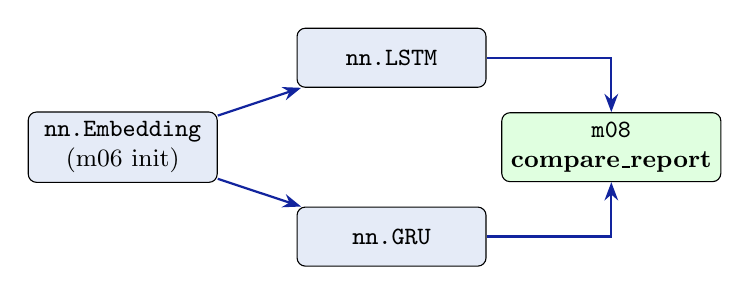
\begin{tikzpicture}[
      mod/.style={draw, fill=cnubluebg, rounded corners=3pt,
                  minimum width=2.4cm, minimum height=0.75cm,
                  font=\small, align=center},
      fin/.style={draw, fill=green!12, rounded corners=3pt,
                  minimum width=2.6cm, minimum height=0.75cm,
                  font=\small\bfseries, align=center},
      arr/.style={-{Stealth}, thick, color=cnublue}
  ]
    \node[mod] (em) {\texttt{nn.Embedding}\\ (m06 init)};
    \node[mod, above right=0.3cm and 1.0cm of em]  (ls) {\texttt{nn.LSTM}};
    \node[mod, below right=0.3cm and 1.0cm of em]  (gr) {\texttt{nn.GRU}};
    \node[fin, right=3.6cm of em]  (m8) {\texttt{m08}\\ compare\_report};
    \draw[arr] (em)--(ls); \draw[arr] (em)--(gr);
    \draw[arr] (ls)-|(m8); \draw[arr] (gr)-|(m8);
  \end{tikzpicture}
  \end{center}
  \vspace{5pt}
  \begin{columns}[T]
    \begin{column}{0.50\textwidth}
      \textbf{P8 da qurasiz:}\\[3pt]
      \small
      \begin{itemize}\setlength\itemsep{2pt}
        \item \texttt{m08 GRULSTMClassifier}: \texttt{arch='lstm'} / \texttt{'gru'}
        \item Bir xil vazifada F1 va tezlik taqqoslash
        \item LSTM forget gate $f_t$ ni tekshirish
      \end{itemize}
    \end{column}
    \begin{column}{0.46\textwidth}
      \textbf{Birinchi assert (bu slayd [I3]):}\\[4pt]
      \small\ttfamily
      assert abs(f\_t - 0.818)\\
      \phantom{xx}< 1e-3\\[4pt]
      \normalfont\footnotesize\color{halfgray}
      \textit{\# Ma'ruza L8 [I3]-slayd bilan}\\
      \textit{\# solishtiring (forget gate)}
    \end{column}
  \end{columns}
\end{frame}

% ----------------------------------------------------------------
% [R] ADABIYOTLAR
% ----------------------------------------------------------------
\begin{frame}{Adabiyotlar}
  \begin{enumerate}\small\setlength\itemsep{5pt}
    \item Hochreiter, S., Schmidhuber, J.\ (1997). \textit{Long Short-Term Memory.}
          Neural Computation 9(8):1735--1780.
    \item Cho, K., va boshq.\ (2014). \textit{Learning Phrase Representations using
          RNN Encoder-Decoder...} EMNLP 2014. (GRU.)
    \item Chung, J., va boshq.\ (2014). \textit{Empirical Evaluation of Gated
          Recurrent Neural Networks on Sequence Modeling.} (GRU vs LSTM.)
    \item Jurafsky, D., Martin, J.H.\ (2023). \textit{Speech and Language
          Processing}, 3-nashr. 9-bob: LSTM va GRU.
    \item \texttt{torch.nn.LSTM} / \texttt{torch.nn.GRU} hujjatlari.
  \end{enumerate}
\end{frame}

% ================================================================
% [S] ILOVALAR (appendix --- slayd soniga kirmaydi)
% ================================================================
\appendix

\begin{frame}{Ilova S1: GRU --- LSTM ning soddalashtirilgani}
  \small
  GRU LSTM dan ikki soddalashtirishda farq qiladi:
  \begin{itemize}\setlength\itemsep{2pt}
    \item Cell state $c_t$ va yashirin holat $h_t$ \textbf{birlashtirilgan} (bitta $h_t$).
    \item Forget va input darvozalari \textbf{bitta} update gate $z_t$ ga birlashtirilgan:
          $h_t=(1-z_t)h_{t-1}+z_t\tilde{h}_t$.
  \end{itemize}
  \bunda{shu sababli GRU da 3 ta blok (z,r,$\tilde{h}$), LSTM da 4 ta (f,i,o,$\tilde{c}$).}
  \vspace{4pt}

  Natija: kamroq parametr, tezroq o'qish; ko'p vazifada sifat farqi kichik.
\end{frame}

\begin{frame}{Ilova S2: forget gate bias'ini musbat boshlash}
  \small
  Amaliy hiyla: $b_f$ ni $+1$ (yoki $+2$) bilan boshlash $\Rightarrow$ boshida
  $f_t=\sigma(\text{katta})\approx 1$, ya'ni model dastlab xotirani \textbf{saqlashga}
  moyil.
  $$ f_t = \sigma(W_f[h_{t-1},x_t] + b_f), \quad b_f = +1 $$
  \bunda{musbat bias o'qitish boshida vanishing gradientni yanada kamaytiradi ---
  Jozefowicz va boshq.\ (2015) tavsiyasi.}
  \vspace{4pt}

  Bu kichik o'zgartirish uzoq ketma-ketliklarda o'qishni sezilarli tezlashtiradi.
\end{frame}

\end{document}
